\documentclass[a4paper]{article}

%% Language and font encodings
\usepackage[english]{babel}
\usepackage[utf8x]{inputenc}
\usepackage[T1]{fontenc}

%% Sets page size and margins
\usepackage[a4paper,top=3cm,bottom=2cm,left=3cm,right=3cm,marginparwidth=1.75cm]{geometry}

%% Useful packages
\usepackage{amsmath}
\usepackage{graphicx}
\usepackage[colorinlistoftodos]{todonotes}
\usepackage[colorlinks=true, allcolors=blue]{hyperref}
\usepackage{listings}
\usepackage{babel}
\usepackage{xcolor}
\lstset { %
    language=C++,
    backgroundcolor=\color{black!5}, % set backgroundcolor
    basicstyle=\footnotesize,% basic font setting
}

\title{Face Detection using Principal Component Analysis}
\author{
  Wåreus, Emil\\
  \texttt{emil.wareus47@gmail.com}
  \and
  Yang, Joe Yizhou\\
  \texttt{n1702894c@e.ntu.edu.sg}
  \and
  Demeules, Antoine\\
  \texttt{N1703169F@e.ntu.edu.sg}
}
\begin{document}
\maketitle

\begin{abstract}
This short paper will cover how real-time face detection was achieved through the use of Principal  Component Analysis. The project was a part of the course \textit{Intelligent System Design} at \textit{Nanyang Technological University} in Singapore. 
\end{abstract}

\section{Introduction}

Image analysis, pattern recognition and machine learning is a hot topic in the modern world of software engineering. Detecting faces and classifying them to a pre-trained dataset is a feature of many known applications today, such as Facebook, Microsoft-Hello and in Apple products. 
\\
The goal of this project is to: 
\begin{enumerate}
\item Successfully find faces in images using Haar-detection with OpenCV
\item Classify the faces to a pre-trained dataset using Principal Component Analysis (PCA)
\item Collect more faces and re-train the PCA
\end{enumerate}


\section{Method}

\subsection{Face-detection with Haar-like features}
For this section of the project, the built in functionality in OpenCV was used. This is a feature to use Haar-like features to detect faces in an image. Through this, the position of each face in the image could be located. This is not optimal, as this method is very sensitive to any variance in the image, such as tilting and distortion. 


\subsection{Face-classification with Principal Component Analysis}

PCA is used for dimensionality reduction of complex data. This makes visualization and classification easier, more invariant and more computationally efficient. In the case of image analysis, each pixel could be viewed as a dimension, and in this project, images are compared with 100x100 pixels. The PCA algorithm will reduces this to $K=200$ dimensions. 
To perform the PCA, the following algorithms was implemented:  
\begin{enumerate}
\item Resizing of each faces in the data set to $100x100$ pixels
\item Flattening of each face-matrix to a $10000x1  (Nx1)$  column vector, as seen in fig \ref{fig:flatten}

\begin{figure}
\centering
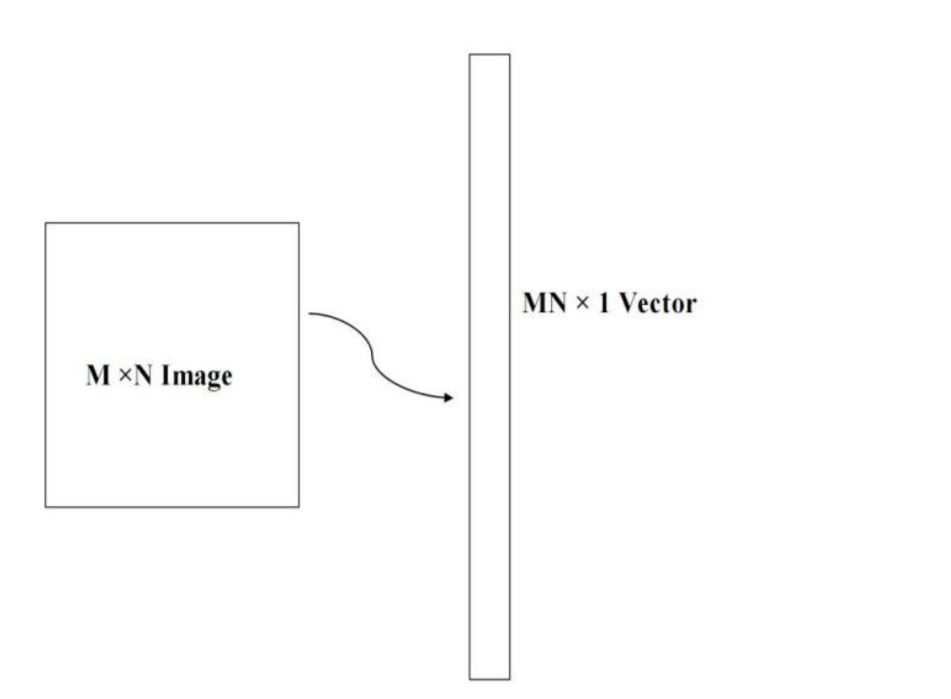
\includegraphics[width=0.3\textwidth]{images/Flatten.JPG}
\caption{\label{fig:flatten}Flattening of matrix to column vector}
\end{figure}


\item Concatenate each column vector $f_1, f_2 ... f_M$, where $M$ is the number of faces in the dataset, to a training matrix $S = [f_1, f_2 ... f_M]$, of size $N x M$
\item The mean face $f_{mean}$ is computed with equation \ref{eqn:fmean} and $S_{mean} = S_n - f_{mean}$. 

\begin{equation}
f_{mean} = \dfrac{1}{M} \sum_{n=1}^{M} f_n
\label{eqn:fmean}
\end{equation}

\item The covariance matrix $C$ is calculated through equation \ref{eqn:cov}. The covariance matrix is of size $N x N$.

\begin{equation}
C = \dfrac{1}{M} \sum_{n=1}^{M} S_{mean, n}S_{mean,n}^T
\label{eqn:cov}
\end{equation}

\item Calculate eigenvalues and eigenvectors. In this project, this is done through the use of the built in functionality of OpenCV, eigen(covariance, eigenvals, eigenvecs). This outputs $M$ eigenvalues, $\lambda_M$, and a $M x M$ matrix of eigenvectors, $\upsilon$. 

\item To perform dimensionality reduction, only the K number of largest eigenvalues $\lambda_{1..K}$ and the corresponding $\upsilon_{K}$ are used. $\upsilon_{K}$ is of dimension $K x M$ and is also called eigenfaces. 

\item To build a comparable dataset of face-weights, a matrix $\Omega$ is introduced in \ref{eqn:faceweights}.

\begin{equation}
\Omega = S_{mean}*\upsilon_{K}^T
\label{eqn:faceweights}
\end{equation}

\item To do a classification, a new face is resized to a Nx1 column vector, $I$. The mean faces is subtracted from $I$ and matrix-multiplied with the eigenfaces. 

\begin{equation}
I_{weight} = (I-f_{mean})^T*\upsilon_{K}^T
\label{eqn:faceweights}
\end{equation}

\item The $I_{weight}$ is then compared with euclidean distance to the face-weights and a minimum distance is computed as in equation \ref{eqn:eucdist}

\begin{equation}
Label = IndexOfMin(\sqrt{\sum (\Omega_{m}-I_{weight})^2})
\label{eqn:eucdist}
\end{equation}

\end{enumerate}	

\section{Implementation And Discussion}
\subsection{Training}

The main training function is dealt with in the \textit{\texttt{train\_pca}} function. Images are read from a directory and then resized into a 100x100 grayscale image which is unrolled into a column vector. The vectors are converted as \texttt{CV\_32F} OpenCV matrices and combined to a feature matrix. PCA is then performed by subtracting the mean for each pixel value for all of the training images. The covariance matrix is calculated as described in 5. The \textit{cv::eigen()} function is used to compute the eigenvectors of the covariance matrix which are already sorted in descending order based on eigenvalue. The top 200 eigenvectors are taken as column vectors, and concatenated, after which the reprojections of the images onto the eigenspace is calculated.
\par
It was noticed that using the the \textit{cv::eigen()} function performs significantly slower than the in-built \textit{cv::PCA()} implementation of PCA. However, our implementation does not require too long for training, and this can be performed ahead of time.

\subsection{Recognition}
There are two phases to the facial recognition system: 
\begin{enumerate}
\item Computing the eigen-face of the test image.
\\
This is done through the function \texttt{\textit{get\_eigen\_face(Mat input\_face, Mat eigenspace)}}, which takes an input matrix of the face and a matrix of eigen-vectors saved in the training process. The \textit{meanface} is subtracted from the input and the multiplied by the eigenspace. This converts the 1x10000 column input face to a 1x200 \textit{eigen-face}.

\item Defining the class with a Nearest Centre Classifier.
\\
In order to improve computation time and also improve the algorithm, a nearest centre classifier is used to compare the input face with the nearest centroid for each class. The centroids for each class are computed ahead of time by taking the centroid across the 200 eigenspace dimensions. 
The \textit{eigen-face} is compared by euclidean distance in the function \texttt{\textit{euclidean\_distance(saved\_eigen\_faces, test\_face)}} to the pre-trained \textit{eigen-face} centroids. The class-label with the minimal distance is returned. This part could have benefited from a more sophisticated algorithm to increase the accuracy, such as a Support Vector Machine (SVM). Our implementation of this is able to run in real time with the face detection, the efficiency of which changes depending on the power of the machine it is running on.
\end{enumerate}


\section{How to use the project}
The file  \texttt{\textit{face\_rec\_training.cpp}} contains two public functions; \texttt{\textit{init()}} and \texttt{\textit{detect\_face(Mat face)}}:
\begin{lstlisting}
/**
Initializes the face recognition with Principal Component analysis. 
The user is asked via cmd to 
1: Retrain the PCA on the images in "/train_images/"
    Then save the trained algorithm or not.
2: Load the pre-trained PCA
*/
void init();

/**
@face: graysclae Mat of face detected with Haar-like features. 
@returns: string containning label of the face
*/
String detect_face(Mat face);
\end{lstlisting}

\section{Results}

A qualitative example is shown below for the face detection using our faces as the detection target. The dataset contains 20 faces with 5 images each contained in the \textit{train\_images} folder, and the recognition determines the closest matching class based on the centroids and displays it on top of the image. 

\begin{figure}[b]
\centering
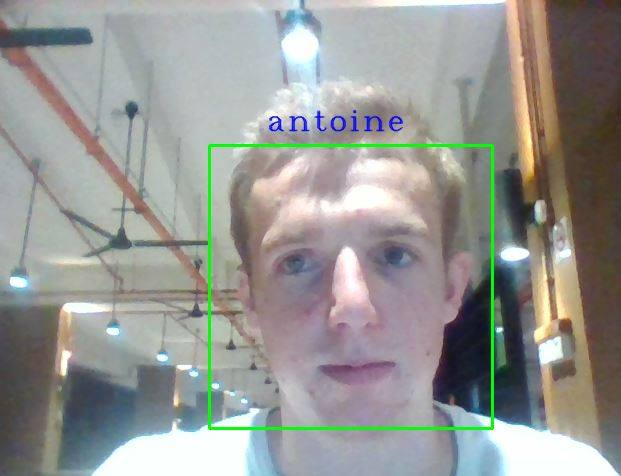
\includegraphics[width=0.35\textwidth]{images/detection1.jpg}
\caption{\label{fig:detetion}Example of recognition, the name is displayed on top.}
\end{figure}

\end{document}